\documentclass[11pt;a4paper]{report}
\usepackage[free-standing-units]{siunitx}
\usepackage{circuitikz}
\usepackage{tikz}
\usepackage[utf8]{inputenc}
\usepackage{fontenc}
\usepackage[french]{babel}
\usepackage{lmodern}
\usepackage{amsmath}
\usepackage{amssymb}
\usepackage{mathrsfs}
\usepackage[top=2cm, bottom=2cm, left=2cm, right=2cm]{geometry}
\usepackage{multirow}
\usepackage{url,hyperref}
\usepackage{siunitx}
\usepackage{schemabloc}

\title{
\includegraphics{../../../images/inp-enseeiht} \\ ~ \\ ~ \\ ~ \\ ~ \\ Mini Projet Électronique Linéaire \\ ~ \\ \large{Réalisation d'un amplificateur de tension}}
\author{Mathieu Morino, Guilhem Saurel}
\date{\oldstylenums{\today}}

\renewcommand{\thechapter}{\Roman{chapter}}
\renewcommand{\thesection}{\thechapter .\Alph{section}}

\begin{document}
 \begin{titlepage}
  \maketitle
 \end{titlepage}


 %\hspace{30mm}
 \tableofcontents


 \chapter{Énoncé}
  \section{Cahier des charges}

    \begin{tabular}{|l|l|c|c|c|c|c|}
     \hline
     & & Typique & Tolérance & Minimum & Maximum & Unités \\
     \hline
     \multirow{4}{3cm}{Caractéristiques générales à 30k\hertz} & Gain en tension & 60 & $\pm$ 5dB & 55 & 65 & dB \\
     \cline{2-7} & Résistance d'entrée & 30 & $\pm$ 15 \% & 25.5 & 34.5 & \kilo\ohm \\
     \cline{2-7} & Résistance de sortie & 100 & $\pm$ 15 \% & 85 & 115 & \ohm \\
     \cline{2-7} & Dynamique de sortie & & & 6 & & V càc \\
     \hline
     \multirow{2}{3cm}{Fréquence de coupure} & basse & 100 & $\pm$ 20 \% & 80 & 120 & \hertz \\
     \cline{2-7} & haute & & & 500 & & k\hertz \\
     \hline
     Distorsion harmonique & [1k\hertz;100k\hertz] & & & & 1,00 \% & \\
     \hline
     \multirow{2}*{Tension d'alimentation} & Positive & 12V & & 0 & 12 & V \\
     \cline{2-7} & Négative & -12V & & -12 & 0 & V \\
     \hline
     Courant de collecteur & & & & 0.1 & 10 & mA \\
     \hline
    \end{tabular}


  \section{Contraintes}
    Obligation d'utiliser un montage d'amplification différentiel.

    Consommer le moins possible.


  \section{Conditions d'utilisation}

    \underline{Entrée} : Générateur basse fréquence de résistance interne $R_g = 50 \ohm$

    \underline{Sortie} : Résistance de charge $R_L = 5\kilo\ohm$


  \section{Composants}
    \underline{Actifs} : Transistors BC238

    \underline{Passifs} : Composants appartenant à la norme E12

    \underline{Valeurs} de la norme E12 : 1 ; 1.2 ; 1.5 ; 1.8 ; 2.2 ; 2.7 ; 3.3 ; 3.9 ; 4.7 ; 5.6 ; 6.8 ; 8.2

    \begin{tabular}{|c|c|c|c|}
     \hline
     & Minimum & Maximum & Unités \\
     \hline
     Résistances & 10 & $10^6$ & \ohm \\
     \hline
     Condensateurs & 10 & $4,7.10^6$ & pF \\
     \hline
    \end{tabular}

    Précisions : À partir de 1 $\micro$F, les condensateurs sont polarisés ( ils ont donc un sens de branchement). 
    Les seules valeurs disponibles sont 1$\micro$F, 2.2$\micro$F et 4.7$\micro$F.


  \section{Calendrier}

    \begin{tabular}{|p{2cm}|p{2cm}|p{12cm}|}
     \hline Début & Fin & Activité \\
     \hline 28/02/2011 & 16/03/2011 & 3 Séances de TD : 
      \begin{itemize}
       \item Faire les calculs théoriques des circuits.
       \item Valider les calculs par des simulations sous Orcad Spice.
       \item Réaliser un rapport intermédiaire.
      \end{itemize} \\
     \hline 21/03/2011 & & Remise des rapports \\
     \hline 28/03/2011 & 31/03/2011 & Retour des rapports intermédiaires corrigés. Inititiation à SPICE PCB \\
     \hline 04/04/2011 & 09/04/2011 & Réalisation des premiers étages de gain sur plaquette Labdec. Tests de polarisation et tracer de diagramme de Bode \\
     \hline 11/04/2011 & 15/04/2011 & Réalisation de la deuxième partie du montage sur plaquette Labdec. Tests de polarisation et tracer de diagramme de Bode \\
     \hline 18/04/2011 & 22/04/2011 & Réalisation du circuit imprimé de l'amplificateur. \\
     \hline 09/05/2011 & 13/05/2011 & Perçage. Soudage du 1\textsuperscript{er} étage de gain. Le caractériser. \\
     \hline 16/05/2011 & 20/05/2011 & Soudage du 2\textsuperscript{ème} étage de gain. Le caractériser. Relier le 1\textsuperscript{er} et le 2\textsuperscript{ème} étage. Caractériser l'amplificateur complet. \\
     \hline 16/05/2011 & 20/05/2011 & Oral à la fin de la dernière séance. \\
     \hline
    \end{tabular}



 \chapter{Études théorique des différents composants}
  \section{Collecteur Commun}
   \subsection{Schéma}

   On utilisera le schéma suivant de collecteur commun :

    \begin{circuitikz} \draw
     (0,3) to[open,v=$V_E$] (0,0)
     (7,2) to[open,v=$V_S$] (7,0)
     (0,0) -- (7,0)
     (0,3) to[C,i=$I_E$] (2,3)
      to [R=$R_{B1}$] (2,6) -- (4,6)
      to [R=$R_C$] (4,4) -- (6,4)
      to [C] (6,6) -- (4,6)
     (4,3) node[npn](npn){}
      (npn.B) -- (2,3)
      (npn.C) -- (4,4)
      (npn.E) -- (4,2)
     (2,3) to [R=$R_{B2}$] (2,0) -- (4,0)
      to [R=$R_E$] (4,2)
      to [C,i=$I_S$] (7,2)
     (1,6) node[anchor=east] {$V_{cc}$} to [short,o-] (2,6)
     ;
    \end{circuitikz}

   \subsection{Polarisation}
    En raison de la présence des condensateurs, ce circuit est équivalent à (en continu) :

    \begin{circuitikz} \draw
     (3,2) to [R=$R_E$] (3,0) -- (0,0)
      to [battery=$E_{th}$] (0,3)
      to [R=$R_B$] (2,3)
     (2,6) node[anchor=east] {$V_{cc}$} to [short,o-] (3,6)
      to [R=$R_C$] (3,4)
     (3,3) node[npn](npn){}
      (npn.B) -- (2,3)
      (npn.C) -- (3,4)
      (npn.E) -- (3,2)
     ;
    \end{circuitikz}

    On a alors les relations suivantes :

    $\left.
      \begin{array}{c}
       R_B = \cfrac{R_{B1} R_{B2}}{R_{B1} + R_{B2}} \\
       E_{th} = \cfrac{V_{cc}}{1+\cfrac{R_{B1}}{ R_{B2}}} \\
       R_E I_C + V_{BE} + R_B I_B = E_{th} \\
       I_C = \beta I_B
      \end{array}
    \right\} \Rightarrow I_C = \cfrac{E_{th} - V_{BE}}{R_E + \cfrac{R_B}{\beta}}$

   \subsection{Droite de charge statique}

    Afin de limiter les effets de distorsion, on s'efforcera de placer le point de polarisation Q au milieu de la droite de charge statique.
    
    $V_{cc} = R_C I_C + V_{CE} + R_E I_C$

    $I_C = \cfrac{V_{cc} - V_{CE}}{R_E+R_C}$

    \begin{circuitikz}
     \begin{scope}[xshift=6.5cm, yshift=.5cm]
      \draw [->] (0,0) -- (4.5,0) node[anchor=west] {$V_{CE} $};
      \draw [->] (0,0) -- (0,2.5) node[anchor=west] {$I_C$} ;
      \draw (2,0) node[anchor=north] {$\cfrac{V_{cc}}{2}$}
            (4,0) node[anchor=north] {$V_{cc}$}
            (0,1) node[anchor=east] {$\cfrac{V_{cc}}{2(R_E+R_C)}$}
            (0,2) node[anchor=east] {$\cfrac{V_{cc}}{R_E+R_C}$}
            (0,0) node[anchor=north] {0};
      \draw [thick] (0,2) -- (4,0);
      \draw [dotted] (0,1) -- (2,1) -- (2,0);
     \end{scope}
    \end{circuitikz}

   \subsection{Schéma équivalent petit signal}
    Aux fréquences moyennes et en comportement petit signal, on obtient le schéma équivalent suivant :

    \begin{circuitikz} \draw
     (0,4) to[open,v=$V_E$] (0,0) -- (11,0)
     (11,2) to[open,v=$V_S$] (11,0)
     (0,4) to [short,i=$I_E$] (1,4) --(5,4)
      to [R=$r_b$,v=v] (5,2) -- (10,2)
      to [short,i=$I_S$] (11,2)
     (1,0) to [R=$R_{B1}$] (1,4)
     (3,0) to [R=$R_{B2}$] (3,4)
     (7,0) to [R=$R_E$] (7,2)
     (9,0) to [cI=$g_mv$] (9,2)
     ;
    \end{circuitikz}

    $g_m = \cfrac{I_C}{U_T}$

    $r_b = \cfrac{\beta}{g_m}$

   \subsection{Droite de charge dynamique}

    $\cfrac{V_{CE}(t)}{I_C(t)} = - R_E \parallel Z_L$

    \begin{circuitikz}
    \begin{scope}[xshift=6.5cm, yshift=.5cm]
     \draw [->] (0,0) -- (4.5,0) node[anchor=west] {$V_{CE}(t) $};
     \draw [->] (0,0) -- (0,2.5) node[anchor=west] {$I_C(t)$} ;
     \draw (3,0) node[anchor=north] {$V_{CE_Q}$}
           (4,0) node[anchor=north] {$V_{CE_{max}}$}
           (0,0.5) node[anchor=east] {$I_{C_Q}$}
           (0,2) node[anchor=east] {$I_{C_{max}}$}
           (0,0) node[anchor=north] {0};
     \draw [thick] (0,2) -- (4,0);
     \draw [dotted] (0,0.5) -- (3,0.5) -- (3,0);
    \end{scope}
    \end{circuitikz}

    Donc dynamique de sortie maximale (crête à crête) = $2(V_{CEmax}-V_{CEQ}) = 2 I_{CQ} (R_E \parallel Z_L)$ car $V_S = -V_{CE}$

   \subsection{Impédance d'entrée}

    $\left.
     \begin{array}{c}
      Z_E = \cfrac{V_E}{I_E}\\
      V_E = v + V_S \\
      v = r_b i \\
      V_S = (R_E \parallel Z_L)(i+g_mv)
     \end{array}
    \right\} 
    \begin{array}{l}
     \Rightarrow \cfrac{V_E}{i}=\cfrac{v+V_S}{i} =r_b + (R_E\parallel Z_L)(1+g_mr_b) \\
     \Rightarrow Z_E = R_B \parallel \left ( r_b + \beta (R_E\parallel Z_L) \right )
    \end{array}$

   \subsection{Impédance de sortie}
    $Z_S = \cfrac{V}{i+g_mv} = R_E\cfrac{i+g_mv-\cfrac{v}{r_b}}{i+g_mv}$

    $Z_S = R_E \parallel (\cfrac{r_b + R_g \parallel R_B}{\beta})$


   \subsection{Gain}

    $a_v = \cfrac{V_S}{V_E} = \cfrac{V_S}{v+V_S} = \cfrac{\beta(R_E \parallel Z_L)}{r_b+\beta(R_E\parallel Z_L)} \approx 1$

    ~

    On considérera donc le gain de cet étage comme égal à 1.


  \section{Émetteur Commun}
   \subsection{Schéma}
    On utilisera le montage émetteur commun suivant :

    \begin{circuitikz} \draw
     (0,3) to[open,v=$V_E$] (0,0)
     (7,4) to[open,v=$V_S$] (7,0)
     (0,0) -- (7,0)
     (0,3) to[C,i=$I_E$] (2,3)
      to [R=$R_{B1}$] (2,6) -- (4,6)
      to [R=$R_C$] (4,4)
      to [C,i=$I_S$] (7,4) 
     (4,3) node[npn](npn){}
      (npn.B) -- (2,3)
      (npn.C) -- (4,4)
      (npn.E) -- (4,2)
     (2,3) to [R=$R_{B2}$] (2,0) -- (4,0)
      to [R=$R_E$] (4,2) -- (6,2)
      to [C] (6,0)
     (1,6) node[anchor=east] {$V_{cc}$} to [short,o-] (2,6)
     ;
    \end{circuitikz}

   \subsection{Polarisation}
    En raison de la présence des condensateurs, ce circuit est équivalent à (en continu) :

    \begin{circuitikz} \draw
     (3,2) to [R=$R_E$] (3,0) -- (0,0)
      to [battery=$E_{th}$] (0,3)
      to [R=$R_B$] (2,3)
     (2,6) node[anchor=east] {$V_{cc}$} to [short,o-] (3,6)
      to [R=$R_C$] (3,4)
     (3,3) node[npn](npn){}
      (npn.B) -- (2,3)
      (npn.C) -- (3,4)
      (npn.E) -- (3,2)
     ;
    \end{circuitikz}

    On obtient donc les relations suivantes :

    $\left.
      \begin{array}{c}
       R_B = \cfrac{R_{B1} R_{B2}}{R_{B1} + R_{B2}} \\
       E_{th} = \cfrac{V_{cc}}{1+\cfrac{R_{B1}}{ R_{B2}}} \\
       R_E I_C + V_{BE} + R_B I_B = E_{th} \\
       I_C = \beta I_B
      \end{array}
    \right\} \Rightarrow I_C = \cfrac{E_{th} - V_{BE}}{R_E + \cfrac{R_B}{\beta}}$

   \subsection{Droite de charge statique}
    De la même façon que précedemment, on s'efforcera de placer notre point de polarisation au milieu de la droite de charge statique :

    $V_{cc} = R_C I_C + V_{CE} + R_E I_C$

    $I_C = \cfrac{V_{cc} - V_{CE}}{R_E+R_C}$

    \begin{circuitikz}
     \begin{scope}[xshift=6.5cm, yshift=.5cm]
      \draw [->] (0,0) -- (4.5,0) node[anchor=west] {$V_{CE} $};
      \draw [->] (0,0) -- (0,2.5) node[anchor=west] {$I_C$} ;
      \draw (2,0) node[anchor=north] {$\cfrac{V_{cc}}{2}$}
            (4,0) node[anchor=north] {$V_{cc}$}
            (0,1) node[anchor=east] {$\cfrac{V_{cc}}{2(R_E+R_C)}$}
            (0,2) node[anchor=east] {$\cfrac{V_{cc}}{R_E+R_C}$}
            (0,0) node[anchor=north] {0};
      \draw [thick] (0,2) -- (4,0);
      \draw [dotted] (0,1) -- (2,1) -- (2,0);
     \end{scope}
    \end{circuitikz}


   \subsection{Schéma équivalent petit signal}
    Aux fréquences moyennes et en comportement petit signal, on obtient le schéma équivalent suivant :

    \begin{circuitikz} \draw
     (0,2) to [short,i=$I_E$] (1,2) -- (5,2)
      to [R=$r_b$,v=v] (5,0) -- (0,0)
     (0,2) to [open,v=$V_E$] (0,0)
     (1,0) to [R=$R_{B1}$] (1,2)
     (3,0) to [R=$R_{B2}$] (3,2)
     (7,2) to [cI=$g_mv$] (7,0)
     (9,2) to [R=$R_C$] (9,0)
     (7,2) -- (9,2)
      to [short,-o,i=$I_S$] (11,2)
      to [open,v=$V_S$] (11,0) -- (5,0)
     ;
    \end{circuitikz}

    $g_m = \cfrac{I_C}{U_T}$

    $r_b = \cfrac{\beta}{g_m}$

   \subsection{Droite de charge dynamique}

    $\cfrac{V_{CE}(t)}{I_C(t)} = - R_C \parallel Z_L$
   
   \begin{circuitikz}
    \begin{scope}[xshift=6.5cm, yshift=.5cm]
     \draw [->] (0,0) -- (4.5,0) node[anchor=west] {$V_{CE}(t) $};
     \draw [->] (0,0) -- (0,2.5) node[anchor=west] {$I_C(t)$} ;
     \draw (3,0) node[anchor=north] {$V_{CE_Q}$}
           (4,0) node[anchor=north] {$V_{CE_{max}}$}
           (0,0.5) node[anchor=east] {$I_{C_Q}$}
           (0,2) node[anchor=east] {$I_{C_{max}}$}
           (0,0) node[anchor=north] {0};
     \draw [thick] (0,2) -- (4,0);
     \draw [dotted] (0,0.5) -- (3,0.5) -- (3,0);
    \end{scope}
    \end{circuitikz}

    Donc dynamique de sortie maximale (crête à crête) = $2(V_{CEmax}-V_{CEQ}) = 2 I_{CQ} (R_C \parallel Z_L)$ car $V_S = V_{CE}$

   \subsection{Impédance d'entrée}

    $Z_E = \cfrac{V_E}{I_E} = R_B\parallel r_b$

   \subsection{Impédance de sortie}

    $Z_S = R_C$

   \subsection{Gain}

    $a_v = \cfrac{V_S}{V_E} = \cfrac{-g_mv(Z_L \parallel R_C)}{v} = -g_m (Z_L\parallel R_C)$

  \section{Amplificateur différentiel}
   \subsection{Schéma}

    \begin{circuitikz} \draw
     (4,0) -- (0,0) to [battery=12V] (0,4)
      to [battery=12V] (0,9) -- (8,9)
     (4,6) node[npn](npn1){}
      (npn1.B) -- (2,6)
      (npn1.C) -- (4,7)
      (npn1.E) -- (4,5)
     (8,6) node[npn,xscale=-1](npn2){}
      (npn2.B) -- (10,6)
      (npn2.C) -- (8,7)
      (npn2.E) -- (8,5)
     (6,3) node[npn](npn3){T3}
      (npn3.B) -- (4,3)
      (npn3.C) -- (6,5)
      (npn3.E) -- (6,2)
     (6,2) to [R=$R_E$] (6,0) -- (4,0)
      to [R=$R_{B2}$] (4,3) -- (4,4)
      to [R=$R_{B1}$] (2,4) -- (0,4)
     (1,6) to [short,i=$I_E$] (2,6)
      to [R=$R_{BP}$] (2,4) -- (2,3)
     (2,3) node[ground]{}
     (4,9) to [R=$R_C$] (4,7)
     (8,9) to [R=$R_C$] (8,7)
     (10,6) -- (10,5)
     (10,3) -- (10,2) node[ground]{}
     (9,3) to [R=$R_{BP}$] (9,5) -- (11,5)
      to [C] (11,3) -- (9,3)
     (4,5) to [R=$R_{EP}$] (6,5) to [R=$R_{EP}$] (8,5)
     (8,7) -- (10,7) to [short,i=$I_S$] (11,7)
     %(6,5) node[anchor=south]{A}
     ;
    \end{circuitikz}

    Afin de fixer identiquement le courant tans les transistors 1 et 2, on utilisera des résistances $R_{BP}$, $R_{EP}$ et $R_C$ de valeurs identiques.

   \subsection{polarisation de T3}
    $R_B = R_{B1} \parallel R_{B2}$

    $E_{th} = \cfrac{V_{cc}}{1+\cfrac{R_{B1}}{R_{B2}}} - 12 $
    
    $I_{C3} = 2 I_{C1}= \cfrac{E_{th} - V_{BE}}{R_E + \cfrac{R_B}{\beta}}$
 
   \subsection{Schéma équivalent petit signal de T3}
    \begin{circuitikz} \draw
     (9,4) node[anchor=west]{A}
     (9,4) to [open,v=$V_S$] (9,0) -- (0,0)
      to [R=$R_B$] (0,4) -- (2,4)
      to [R=$r_{b3}$,v=v] (2,2) -- (7,2)
      to [R=$r_{03}$] (7,4)
     (9,4) to [short,i=$I_S$] (8,4) -- (4,4)
      to [cI,i=$g_mv$] (4,2)
      to [R=$R_E$] (4,0)
     ;
    \end{circuitikz}

    Ce transistor sert à fixer le courant dans les deux autres, on le modélise par la suite par une impédance $Z_{S3}$

   \subsection{Schéma équivalent petit signal}
    \begin{circuitikz} \draw
     (0,6) to [short,i=$I_E$] (1,6)
      to [R=$r_{b_1}$, v=v] (1,4) -- (4,4)
     (4,6) to [cI,i=$g_mv$] (4,4)
     (4,6) -- (6,6) to [R=$R_{C_1}$] (6,3)
     (6,3) node[ground]{}
     (8,3) node[ground]{}
     (8,3) -- (8,6) -- (9,6)
      to [R=$r_{b_2}$] (9,4) -- (12,4)
     (12,6) to [cI,i=$g_mv$] (12,4)
     (12,6) -- (14,6)
      to [R=$R_{C_2}$] (14,3)
     (14,3) node[ground]{}
     (14,6) to [short, i=$I_S$] (15,6)
     (2,4) -- (2,2) -- (11,2) -- (11,4)
     (7,2) to [R=$Z_{S3}$] (7,0)
     (7,0) node[ground]{}
     ;
    \end{circuitikz}

    \begin{circuitikz} \draw
     (0,6) to [short,i=$I_E$] (1,6)
      to [R=$r_{b_1}$,v=v] (1,4) -- (8,4)
     (8,2) to [cI,i=$g_mv$] (8,4)
     (8,2) to [short,i=$I_S$] (9,2)
     (9,0) -- (0,0)
     (2,0) to [R=$R_{C_1}$] (2,2)
      to [cI,i=$g_mv$] (2,4)
     (4,0) to [R=$Z_{S3}$] (4,4)
     (6,4) to [R=$r_{b_2}$,v=v] (6,0)
     (8,0) to [R=$R_{C_2}$] (8,2)
     ;
    \end{circuitikz}

   \subsection{Droite de charge dynamique}
    $V_{CE} + R_C I_C = 2 I_C ( Z_{S3} \parallel r_b)$
    
    $\cfrac{V_{CE}}{I_C} = 2(Z_{S3}\parallel r_b) - R_C$

    \begin{circuitikz}
    \begin{scope}[xshift=6.5cm, yshift=.5cm]
     \draw [->] (0,0) -- (4.5,0) node[anchor=west] {$V_{CE}(t) $};
     \draw [->] (0,0) -- (0,2.5) node[anchor=west] {$I_C(t)$} ;
     \draw (3,0) node[anchor=north] {$V_{CE_Q}$}
           (4,0) node[anchor=north] {$V_{CE_{max}}$}
           (0,0.5) node[anchor=east] {$I_{C_Q}$}
           (0,2) node[anchor=east] {$I_{C_{max}}$}
           (0,0) node[anchor=north] {0};
     \draw [thick] (0,2) -- (4,0);
     \draw [dotted] (0,0.5) -- (3,0.5) -- (3,0);
    \end{scope}
    \end{circuitikz}

    $2(V_{CEmax}-V_{CEQ}) = 2 I_{CQ} (2(Z_{S3} \parallel r_b) -R_C)$ 
    Donc dynamique de sortie maximale (crête à crête) = $2 I_C (Z_{S3} \parallel r_b) - V_{CE}$

   \subsection{Impédance d'entrée}
    $Z_E = 2 r_b$

   \subsection{Impédance de sortie}
    $Z_S = R_C$

   \subsection{Gain}
    Dans les conditions de notre amplificateur différentiel, on obtient un gain 
    $a_v = \cfrac{g_m R_C}{2}$


 \chapter{Architecture}
  \section{Théorie}

    Le cahier des charges nous impose un gain de 60dB et l'utilisation d'un amplificateur différentiel.
    Afin d'éviter de saturer celui-ci, on choisira de décomposer ce gain en deux étages : un amplificateur différentiel et un émetteur commun.

    l'émetteur commun ayant un gain plus faible que l'amplificateur différentiel, on prendra arbitrairement un gain de 25 pour l'émetteur commun et un gain de 40 pour l'amplificateur différentiel (ce qui fait bien un gain de 1000 = 60dB).

    De plus, on nous impose une impédance d'entrée de 30 \kilo\ohm, ce qui nous amène à ajouter un collecteur commun possédant une forte impédance d'entrée en amont de l'émetteur commun.
    Enfin, il nous est également demandé une impédance de sortie de 100\ohm. On utilise donc ici aussi un collecteur commun en sortie de l'amplificateur différentiel ; en effet, celui-ci possède une faible impédance de sortie.

    Si besoin, nous rajouterons ultérieurement des étages d'adaptation d'impédance.


  \section{Schéma bloc récapitulatif}

    \begin{tikzpicture}
     \sbEntree{E}
     \sbBloc{A}{\textbf{CC} : $Z_E$ = 30\kilo\ohm}{E}
     \sbRelier[E]{E}{A}
     \sbBloc{B}{\textbf{EC} : $a_v$ = 25}{A}
     \sbRelier{A}{B}
     \sbBloc{C}{\textbf{AD} : $a_v$ = 40}{B}
     \sbRelier{B}{C}
     \sbBloc{D}{\textbf{CC} : $Z_S$ = 100\ohm}{C}
     \sbRelier{C}{D}
     
     \sbSortie{S}{D}
     \sbRelier[S]{D}{S}
    \end{tikzpicture}



 \chapter{Applications aux différents étages}
  \section{Collecteur commun du premier étage}
    On veut $Z_e = 30\kilo\ohm$, or $Z_e = R_B \parallel (r_b + \beta ( R_E \parallel R_L ) ) = R_B \parallel \beta ( \cfrac{U_T}{I_{CQ}}+R_E \parallel R_L)$
    
    On sait qu'on peut obtenir $R_L \approx 20 \kilo\ohm$ avec l'étage suivant. On fixe $R_B = Z_e = 30\kilo\ohm$.
    
    On veut donc $\beta(\cfrac{U_T}{I_{CQ}} + R_E \parallel R_L) \approx \beta ( R_E \parallel R_L ) \gg R_B$.
    
    Pour les $\beta$ considérés, $R_E \parallel R_L \geq 1\kilo\ohm$ suffit pour réaliser cette condition. 
    
    Or $I_{CQ} = \cfrac{V_{TH}-V_{BE}}{R_E+\cfrac{R_B}{\beta}} \approx \cfrac{V_{TH}-V_{BE}}{R_E}$. On veut fixer Q ( le point de polarisation ) au milieu de la DDCS (droite de charge statique).
    
    On fixe arbitrairement $R_C \approx 0$ pour simplifier les équations. Néanmoins, on prendra $R_C = 100 \ohm$ pour éviter un court-circuit en cas d'erreur.

    \begin{circuitikz}
    \begin{scope}[xshift=6.5cm, yshift=.5cm]
     \draw [->] (0,0) -- (2.5,0) node[anchor=west] {$V_{CE} $};
     \draw [->] (0,0) -- (0,2.5) node[anchor=west] {$I_C$} ;
     \draw (1,0) node[anchor=north] {$\cfrac{V_{cc}}{2}$}
           (2,0) node[anchor=north] {$V_{cc}$}
           (0,1) node[anchor=east] {$\cfrac{V_{cc}}{2(R_E+R_C)}$}
           (0,2) node[anchor=east] {$\cfrac{V_{cc}}{R_E+R_C}$}
           (0,0) node[anchor=north] {0};
     \draw [thick] (0,2) -- (2,0);
     \draw [dotted] (0,1) -- (1,1) -- (1,0);
    \end{scope}
    \end{circuitikz}

    On veut donc $\cfrac{V_{TH} - V_{BE}}{R_E} \approx \cfrac{V_{cc}}{2R_E} \Rightarrow V_{TH} = \cfrac{V_{cc}}{2} + V_{BE} \Rightarrow \cfrac{V_{TH}}{V_{cc}} = \cfrac{1}{2} + \cfrac{V_{BE}}{V_{cc}} \approx 0.55$
    
    Or $\cfrac{V_{TH}}{V_{cc}} = \cfrac{R_{B2}}{R_{B1}+R_{B2}} = 0.55$, ce qui nous conduit à prendre 
    $\left \{
    \begin{array}{c @{=} c}
        R_{B1} & 54500 \\
        R_{B2} & 66500 \\
    \end{array}
    \right.
    \Rightarrow R_B \approx 30\kilo\ohm$.
    On obtient ainsi :
    \begin{itemize}
     \item $I_{CQ} = 0,3mA$ : au milieu de la DDCS et dans le cahier des charges
     \item $Z_E = \left \{ \begin{array}{c} 29.2\kilo\ohm$ pour $\beta = 380 \\ 29.6\kilo\ohm$ pour $\beta = 800 \end{array} \right. \Rightarrow$ dans le cahier des charges
     \item $Z_S = R_E \parallel \cfrac{r_b+R_{B1} \parallel R_{B2} \parallel R_g}{1+\beta} \approx R_E \parallel \cfrac{U_T}{I_{CQ}} \approx 87 \ohm$
     \item $a_v \approx 1$
    \end{itemize}

  \section{Émetteur commun du second étage}

    On veut $Z_E = 20\kilo\ohm$ et $a_v = \pm 25$, or $Z_E = R_B \parallel r_b = R_B \parallel \cfrac{\beta U_T}{I_{CQ}}$
    
    On va donc fixer $R_B = 20 \kilo \ohm$ (on normalisera les résistances par la suite) et essayer d'obtenir $\cfrac{\beta{U_T}}{I_{CQ}} \gg R_B$ pour avoir $Z_E = 20\kilo\ohm$.
    
    Cela nous encourage à choisir $I_{CQ}$ petit. Or $I_{CQ} = \cfrac{V_{TH}-V_{BE}}{R_E+\cfrac{R_B}{\beta}} \approx \cfrac{V_{TH} - V_{BE}}{R_E}$.
    
    Pour placer Q au milieu de la DDCS, on ne peut pas négliger $R_C$ comme précédemment car $R_C$ intervient dans $a_v$.
    
    On choisit donc arbitrairement $R_{B1} = R_{B2} = 40\kilo\ohm$. Ainsi, $V_{TH} = \cfrac{V_{cc}}{2} = 6V$.
    
    On se propose d'avoir $\cfrac{V_{cc}}{R_E + R_C} = I_{CQ_{max}} = 0,4mA$, ce qui implique $R_E + R_C = 30\kilo\ohm$.
    
    Pour bien fixer Q au milieu de la DDCS, on résoud $\cfrac{V_{TH} -V_{BE}}{R_E} = \cfrac{V_{cc}}{2(R_E+R_C)} \Rightarrow \left \{ \begin{array}{c @{=} c} R_E & 26900 \ohm\\R_C&3100\ohm \end{array} \right.$.
    On a ainsi
    \begin{itemize}
     \item $I_{CQ} = 0,2mA$
     \item $a_v = \cfrac{I_{CQ}}{U_T} (R_C \parallel Z_L ) = -25 \Rightarrow R_C \parallel Z_L = 3250\ohm$
     \item $Z_E = \left \{ \begin{array}{c @{=} c} 14236\ohm $pour$ \beta & 380 \\ 16774\ohm $pour$ \beta & 800 \end{array} \right.$
    \end{itemize}

    Puisque $R_C = 3100 \ohm$, on essaiera d'obtenir $Z_L$ très grand pour le prochain étage.

    Compte tenu des mauvaises performances de $Z_E$, on augmente $R_B$(qui n'intervient que dans l'expression de $Z_E$).

    On prendra $R_B = 23500\ohm$, donc $R_{B1}=R_{B2}=47000 \ohm$. On a alors :

    $\left \{ \begin{array}{c} 15924 \ohm $pour$ \beta = 380 \\ 19168 \ohm $pour$ \beta = 800 \end{array} \right.$.

    Avec $Z_L = 20\kilo\ohm$, on obtient $a_v \approx -20,6$, ce qui reste dans les exigences du cahier des charges.


   \section{Amplificateur différentiel du troisième étage}
    Les calculs dépendant de beaucoup de paramètres, nous nous contenterons de simuler leurs effets sur Spice.
    Cependant, on sait que :
    \begin{itemize}
     \item $R_C$ influe directement sur la valeur du gain et de l'impédance de sortie.
     \item On veillera à polariser T3 de façon à ce que les courants de collecteur respectent le cahier des charges.
     \item On essaiera de minimiser ces courants de collecteur de façon à avoir $Z_E$ le plus grand possible pour l'étage précédent.
    \end{itemize}


   \section{Collecteur Commun du dernier étage}
    On prendra les mêmes valeurs pour $R_{B1}$, $R_{B2}$ et $R_C$. En effet, celles-ci sont parfaitement adaptées à une polarisation précise : comme vu précédemment, on place Q au milieu de la droite de charge statique, tout en évitant les erreurs dûes aux courts-circuits grâce à $R_C$.

    On ajuste ensuite la valeur de $R_E$ de façon à avoir la bonne résistance de sortie. Cependant, il est difficilement réalisable d'ajuster $R_E$ de façon à placer Q au milieu de la droite de charge statique et d'obtenir la résitance de sortie désirée.
    Après quelques calculs, on prend $R_E = 4700\ohm$, et on obtient $Z_S = R_E \parallel (\cfrac{r_b + R_g \parallel R_B}{\beta}) = 21\ohm$.
    Cette valeur ne correspondant pas au cahier des charges, on placera une résistance R=79\ohm en série à la sortie de notre amplificateur (qui est bien négligeable de $Z_L = 5\kilo\ohm$). Ainsi, on a bien $Z_S = 100\ohm$.

%  \section{Synthèse des deux premiers étages}
%   \subsection{Schéma équivalent petit signal}
%
%    \begin{circuitikz} \draw
%     (1,4) to [open,v=$V_E$,color=red] (1,0)
%     (1,0) to [short,color=red] (0,0)
%      to [sV=e,color=red] (0,2)
%      to [R=$R_g$,color=red] (0,4)
%      to [short,color=red,i=$I_E$] (1,4)
%      to [short,color=blue](4,4)
%      to [R=$R_2$,color=blue,v=$v_1$] (4,2)
%      to [short,color=blue] (7,2)
%      to [short,color=green] (8,2)
%      to [R=$R_4$,color=green,v=$v_2$] (8,0)
%      to [short,color=green] (7,0)
%      to [short,color=blue] (1,0)
%     (2,0) to [R=$R_1$,color=blue] (2,4)
%     (4,0) to [R=$R_3$,color=blue] (4,2)
%     (6,0) to [cI=$g_{m1}v_1$,color=blue] (6,2)
%     (10,2) to [short,color=green] (13,2)
%      to [short,i=$I_S$,color=green] (14,2)
%      to [open,v=$V_S$,color=green] (14,0)
%      to [short,color=green] (8,0)
%     (10,2) to [cI=$g_{m2}v_2$,color=green] (10,0)
%     (12,2) to [R=$R_5$,color=green] (12,0)
%     ;
%    \end{circuitikz}
%  
%    $R_1 = R_{B_1}$ 
%  
%    $R_2 = r_{b_1}$
%    
%    $R_3 = R_{E_1}$
%    
%    $R_4 = R_{B_2} \parallel r_{b_2}$
%    
%    $R_5 = R_{C_2}$
%  
%   \subsection{Impédance d'entrée}
%    $Z_E = R_1 \parallel (R_2 + \beta(R_3 \parallel R_4))$
%  
%   \subsection{Impédance de sortie}
%    $Z_S = Z_L \parallel R_5$
%  
%   \subsection{Gain}
%    $G_V = \cfrac{V_S}{e}= \cfrac{V_S}{V_E + R_g I_E} = \cfrac{V_S}{V_E(1+\cfrac{R_g}{Z_E})} \approx {a_v} = -g_{m1} \cfrac{\beta_1(R_3 \parallel R_4)(R_5\parallel Z_L)}{R_2+(R_3\parallel R_4)\beta_1}$
%  
%  

   \section{\textit{Nota Bene}}
    Nos calculs semblent cohérents, mais nous aurons très probablement besoin de faire des ajustements lors de la simulation sous Spice.



 \chapter{Simulation sous Orcad Spice}
  \section{Circuit}
    Puisque notre amplificateur est composé de quatre étages indépendants, nous avons décidé d'utiliser quatre "pages"
    différentes, ainsi qu'une "page"  principale, regroupant les différents circuits précédents, afin d'y voir plus clairement.

    \emph{NB} : Certains composants utilisés dans ces schémas ne respectent pas la norme E12, mais sont néanmoins nécessaires.
    Nous utiliserons donc des combinaisons d'autres composants :
    \begin{itemize}
     \item $54,5 \kilo \ohm = 120 \kilo\ohm \parallel 100 \kilo\ohm$
     \item $66.5 \kilo \ohm = 120 \kilo\ohm \parallel 150 \kilo\ohm$
     \item $20 \kilo\ohm = 10 \kilo\ohm + 10 \kilo\ohm$
     \item $9.4 \micro \farad = 4.7 \micro\farad \parallel 4.7 \micro\farad$ 
    \end{itemize}

   \subsection{Page principale}
    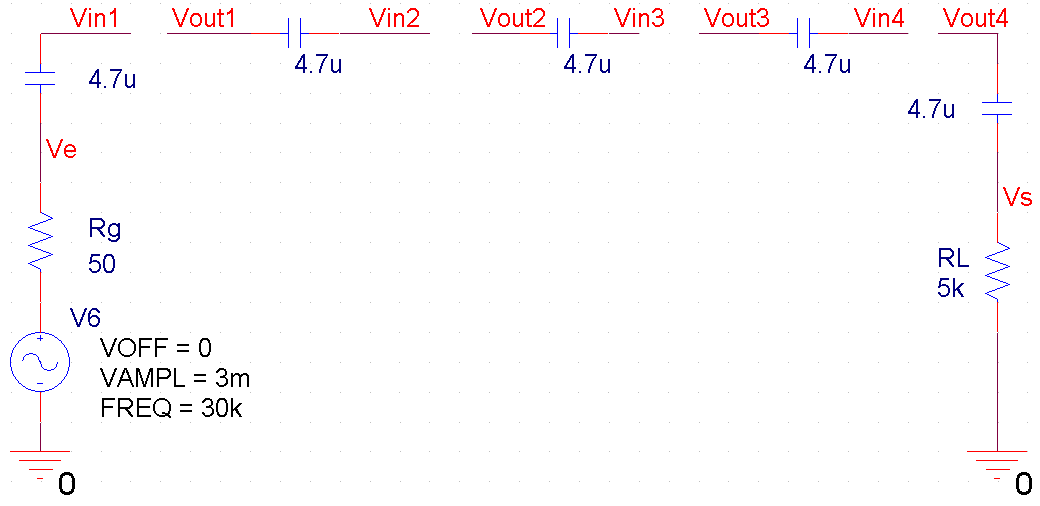
\includegraphics[width=18cm]{images/circuit_main}
    On choisit les autres condensateurs de manière à nous assurer une fréquence de coupure voisine de 100 \hertz.

   \subsection{Premier étage : Collecteur Commun}
    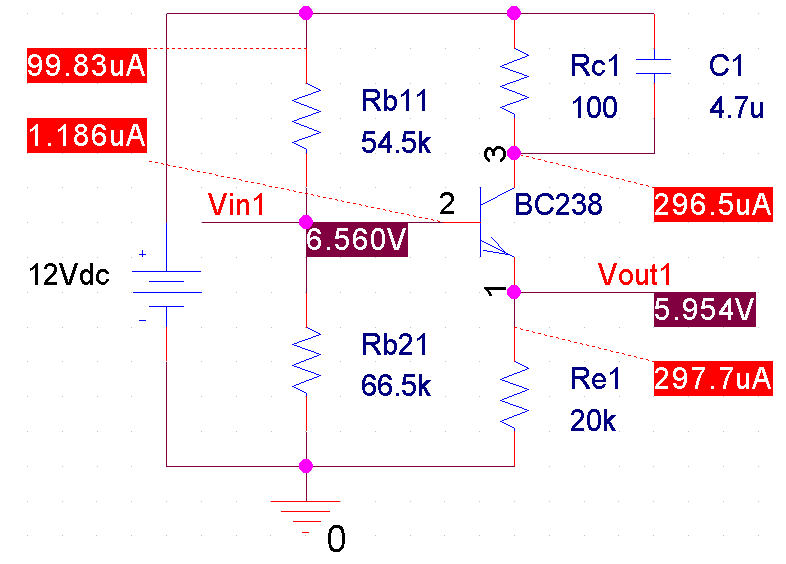
\includegraphics[width=18cm]{images/circuit_1}

   \subsection{Deuxième étage : Émetteur Commun}
    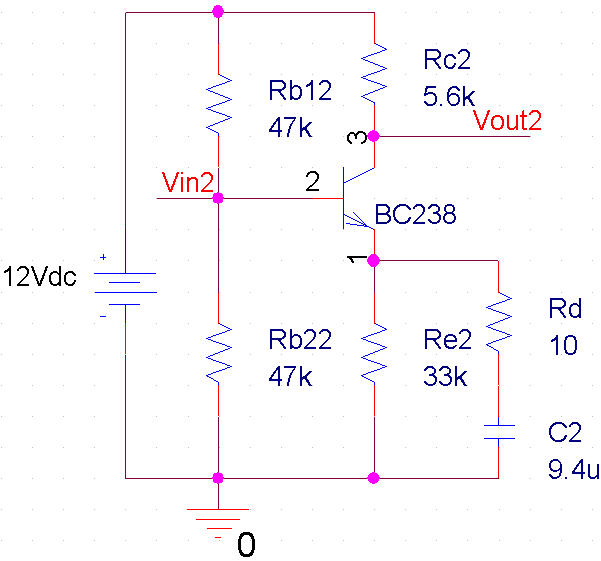
\includegraphics[width=18cm]{images/circuit_2}

    Après une première simulation sous Spice, nous nous sommes rendus compte que la fréquence de coupure basse n'était pas respectée.
    Pour cette raison, on ajoute la résistance $R_d$ en série avec le condensateur (celle-ci ne modifie pas la polarisation) afin de diminuer cette fréquence.
    Cependant, cette résistance a un fort impact négatif sur le gain, nous sommes donc amenés à augmenter la valeur du condensateur. On utilisera donc $C=9,4 \micro\farad$  ce qui correspond à deux condesateurs de 4,7 \micro\farad  en parallèle.

   \subsection{Troisième étage : Amplificateur Différentiel}
    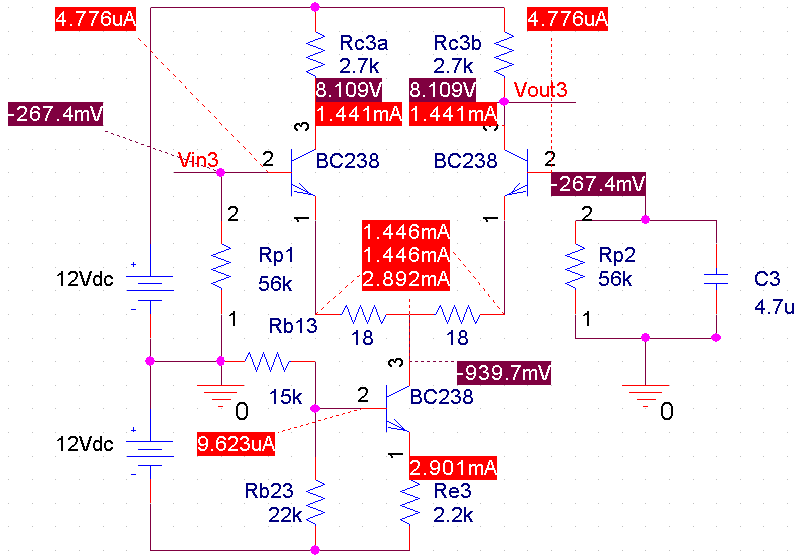
\includegraphics[width=18cm]{images/circuit_3}

    Pour cet étage, on choisira une résistance $R_p$ importante afin d'avoir un gain maximum.
    En effet celle-ci est en parallèle avec la résistance d'entrée de l'émetteur commun.

    Étant donné les mauvaises performances obtenues sur la distorsion après une première simulation, on choisit d'ajouter deux résistances de 18 \ohm  sur l'émetteur des transistors T1 et T2. Ces résistances diminuent fortement la distorsion, mais ont aussi un impact négatif très important sur le gain.

   \subsection{Quatrième étage : Collecteur Commun}
    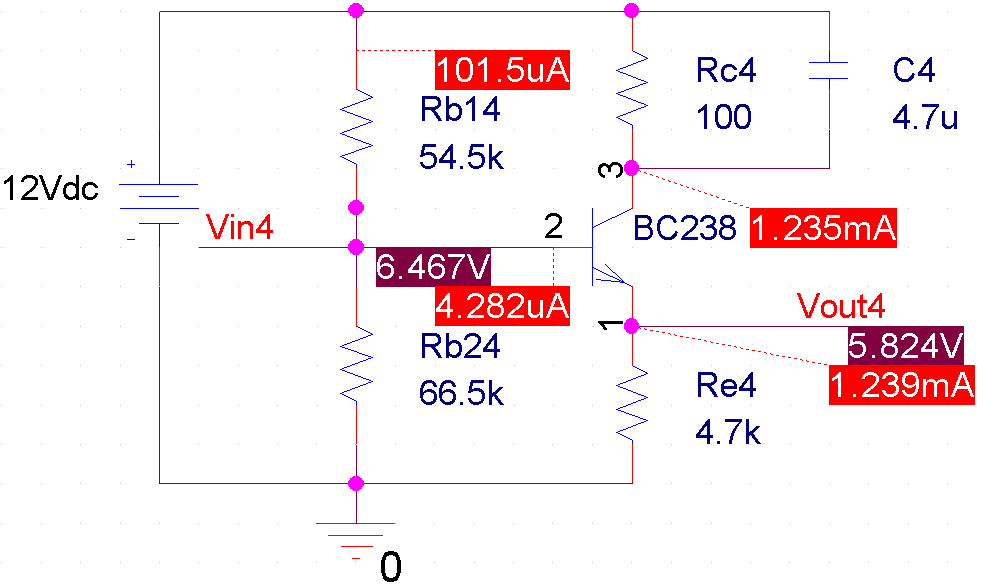
\includegraphics[width=18cm]{images/circuit_4}

  \section{Simulation}
   \subsection{Réponse temporelle à 30\kilo\hertz}
    On trace la courbe de $V_S$ en fonction du temps, et on obtient le graphe suivant, possédant une dynamique de sortie de 5,98 \volt :
    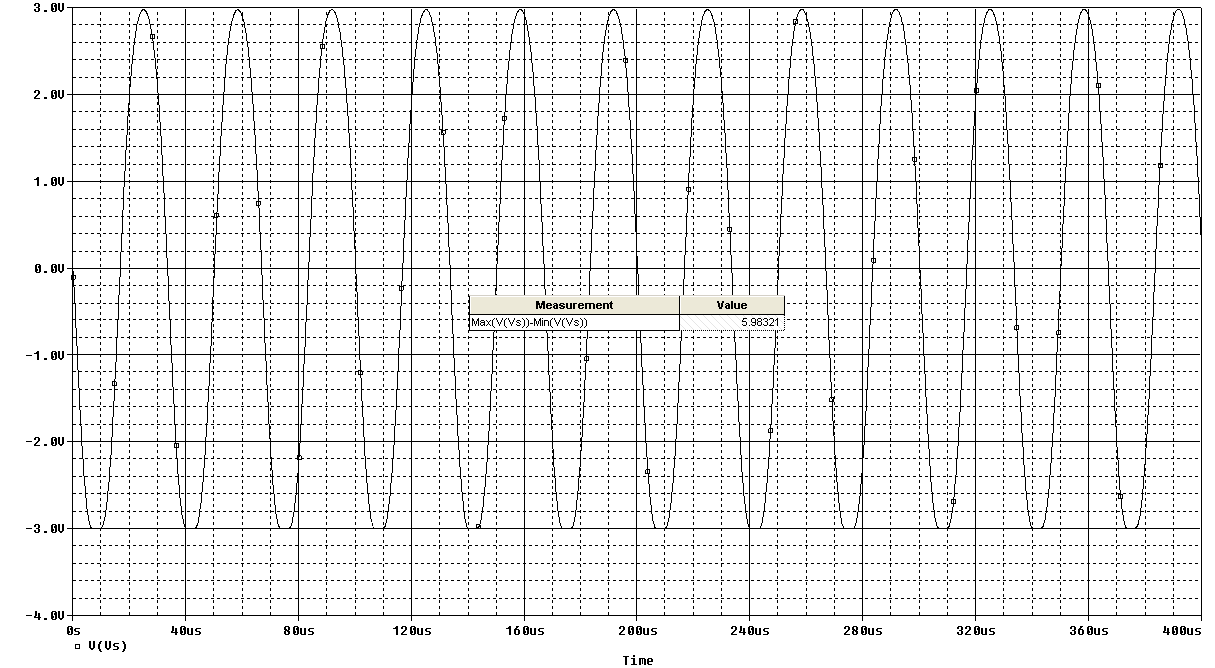
\includegraphics[width=18cm]{images/reponse_temporelle}
    
   \subsection{Diagramme de Bode}
    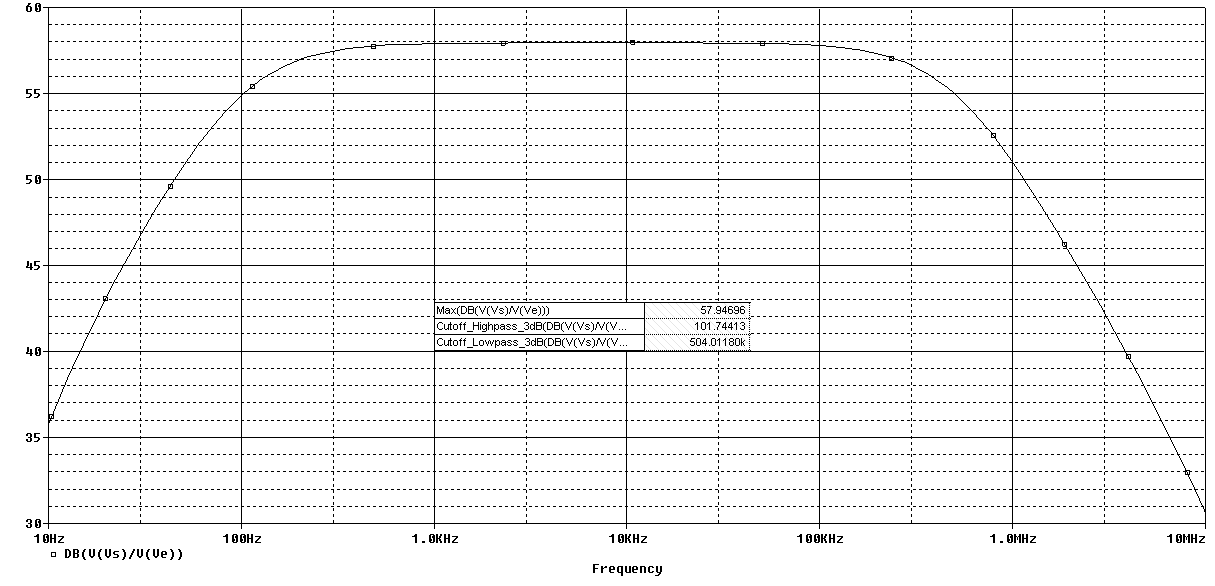
\includegraphics[width=18cm]{images/bode}

   \subsection{Transformée de Fourier}
    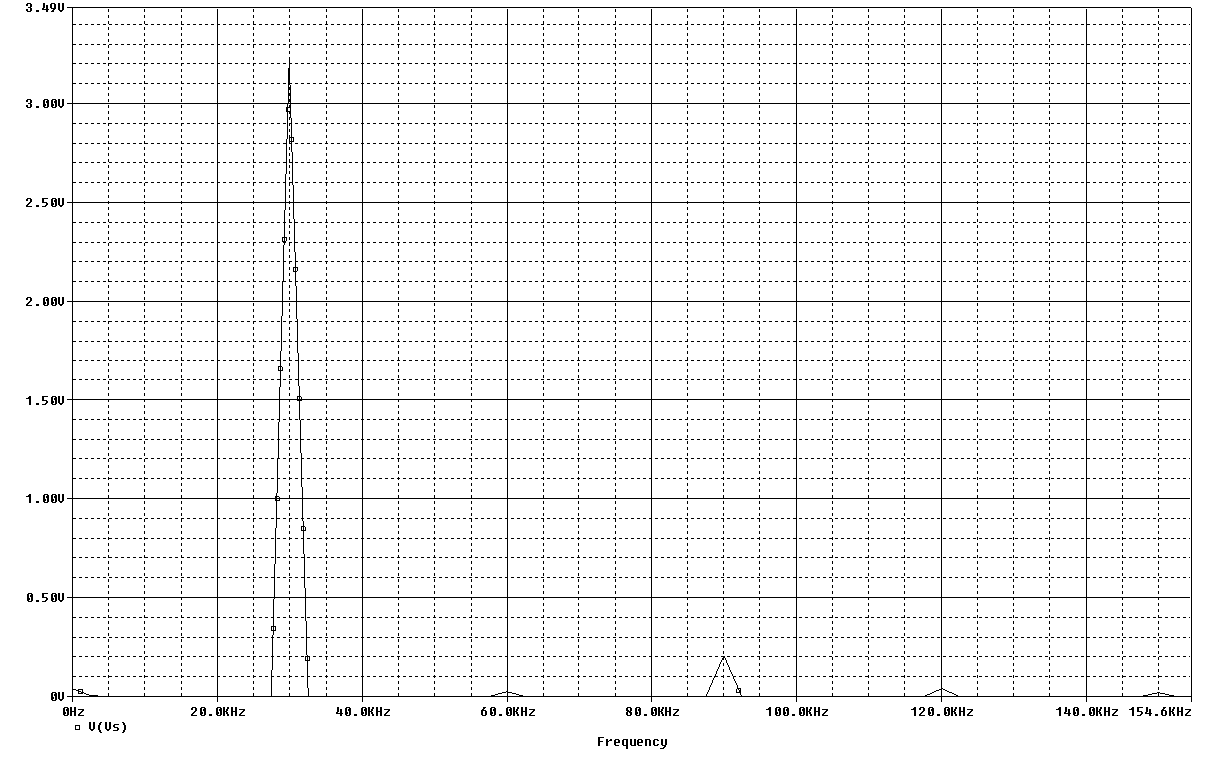
\includegraphics[width=18cm]{images/fft}

  \section{Respect du cahier des charges}
   \subsection{Fréquences de coupure}
    Ces fréquences sont données par Spice avec les fonctions \verb|Cutoff_Lowpass_3dB()| et \verb|Cutoff_Highpass_3dB()| :

    $F_{CBF} = 101$ \hertz

    $F_{CHF} = 504$ \kilo\hertz

   \subsection{Impédances d'entrée et de sortie}
    En traçant un "diagramme de Bode" sous Spice avec, pour chaque étage, $\cfrac{V_E}{I_E}$, on obtient (à 30 \kilo\hertz):
    \begin{itemize}
     \item $Z_{E_1} = \verb|29658|\ohm = Z_E$ : On respecte bien le cahier des charges.
     \item $Z_{E_2} = \verb|15034|\ohm$
     \item $Z_{E_3} = \verb|16107|\ohm$
     \item $Z_{E_4} = \verb|28788|\ohm$
    \end{itemize}

    Pour l'impédance de sortie, il faut modifier un peu le circuit sous spice : court-circuiter l'entrée et déplacer le générateur à la place de la charge. On obtient alors :
    \begin{itemize}
     \item $Z_{S_1} = \verb|191|\ohm$
     \item $Z_{S_2} = \verb|5390|\ohm$
     \item $Z_{S_3} = \verb|2690|\ohm$
     \item $Z_{S_4} = \verb|113|\ohm = Z_S \Rightarrow$ Contrairement à ce que nous avions prévu, nous n'ajouterons pas de résistance série.
    \end{itemize}

   \subsection{Gain et dynamique de sortie}
    On obtient un gain de 57.9 dB, soit une amplification de 785.
    Donc pour une dynamique de sortie de 6V, il faut une tension d'entrée de 3.8 \milli\volt.
    Or on obtient ladite dynamique de sortie avec 4.8 \milli\volt  sous Spice. Ceci est dû à une légère distorsion sur le collecteur commun du dernier étage (cf. paragraphe suivant).
   
   \subsection{Distorsion harmonique}
    Toujours d'après Spice : \verb|TOTAL HARMONIC DISTORTION =   6.668896E+00 PERCENT|

   \subsection{Courants de collecteur}
    \begin{itemize}
     \item $I_{C_1} = 0,296 \milli\ampere$
     \item $I_{C_2} = 0,162 \milli\ampere$
     \item $I_{C_3} = 1,441 \milli\ampere$
     \item $I_{C_4} = 1,235 \milli\ampere$
    \end{itemize}

   \subsection{Amplitudes crête à crête}
    \begin{itemize}
     \item $A_1 =$ \verb|9,48m| \volt
     \item $A_2 =$ \verb|242,3m| \volt
     \item $A_3 =$ \verb|5,99| \volt
     \item $A_4 =$ \verb|6,24| \volt
    \end{itemize}

 \chapter{Bilan}
  \section{Respect du cahier des charges}
     \begin{tabular}{|l|l|c|c|c|c|c|c|}
     \hline
     & & Typique & Tolérance & Minimum & Maximum & Unités & Obtenu \\
     \hline
     \multirow{4}{3cm}{Caractéristiques générales à 30k\hertz} & Gain en tension & 60 & $\pm$ 5dB & 55 & 65 & dB & 57.95\\
     \cline{2-8} & Résistance d'entrée & 30 & $\pm$ 15 \% & 25.5 & 34.5 & \kilo\ohm & 29.658\\
     \cline{2-8} & Résistance de sortie & 100 & $\pm$ 15 \% & 85 & 115 & \ohm & 113\\
     \cline{2-8} & Dynamique de sortie & & & 6 & & V càc & 5.98\\
     \hline
     \multirow{2}{3cm}{Fréquence de coupure} & basse & 100 & $\pm$ 20 \% & 80 & 120 & \hertz & 101 \hertz \\
     \cline{2-8} & haute & & & 500 & & k\hertz & 504 \\
     \hline
     Distorsion harmonique & [1k\hertz;100k\hertz] & & & & 1,00 & \% & 6.67 \\
     \hline
     \multirow{2}*{Tension d'alimentation} & Positive & 12V & & 0 & 12 & V & 12\\
     \cline{2-8} & Négative & -12V & & -12 & 0 & V & -12\\
     \hline
     Courant de collecteur & & & & 0.1 & 10 & mA & OK\\
     \hline
    \end{tabular}

 


\end{document}
%TODO encadrer
